\chapter{Resultat}
\textit{I dette kapitel beskrives resultatet for evaluering af systemets anvendelighed i forhold til at besvare problemformuleringen.}

\section{Sammenligning af risikoscore og rangering}
Systemets anvendelighed er evalueret af 11 medarbejdere fra forskellige afdelinger på SRN, herunder otte fra Lægemiddelinformation og tre fra Klinisk Farmaci. Ud fra vurderingerne, foretaget af medarbejderne, er der defineret en Golden Standard. Denne er bestemt ud fra, at over 60~\% af medarbejderne er enige i, at et lægemiddelskift kræver uddybende information, hvilket fremgår af de individuelle vurderinger af medarbejderne i Tabel \ref{table:resultat} i Appendiks \ref{App:Resultat}.

Ud af 33 lægemiddelskift er 19 vurderet af seks medarbejdere til at skulle have enten lavere eller højere risikoscore end systemets risikovurdering, hvilket fremgår af Tabel \ref{table:resultat3} i Appendiks \ref{App:Rang}. Ud af disse vurderinger er tre eller fire medarbejdere enige i, at tre lægemiddelskift kræver en lavere risikoscore, hvor de resterende 16 lægemiddelskift varierer, mellem at én eller to medarbejdere har vurderet disse til en lavere score. %Denne variation kan skyldes, at medarbejderne er repræsenteret fra forskellige afdelinger og derved har forskellige vurderinger af lægemiddelskiftene, samt at deres erfaring har indflydelse på, hvordan lægemiddelskiftet er vurderet. 
For at evaluere risikoscoren og rangeringen af denne sammenlignes vurderingerne af Lægemiddel Nyt og medarbejderne, angivet som Golden Standard, hvilket fremgår af Tabel \ref{table:test2}. 

\vspace{0.5cm}
\begin{longtable}{|l|c|c|c|c|c|c|c|c|c|c|c|c|c|c|c|c|c|}
\caption{Vurdering af lægemiddelskift for Lægemiddel Nyt og medarbejderne, angivet som Golden Standard. En vurdering til nej betyder, at et lægemiddelskift ikke kræver uddybende information, og en vurdering til ja betyder, at et lægemiddelskift kræver uddybende information. Vurdering under 60~\% enighed mellem medarbejderne er markeret med rødt. Uenighed mellem Lægemiddel Nyt og medarbejderne er markeret med grønt, hvor uenighed mellem lægemiddelskift med samme risikoscore er markeret med blåt ved den pågældende risikoscore.}
	\label{table:test2} \\ \hline
\rowcolor[HTML]{C0C0C0} \textbf{} & \multicolumn{11}{|c|}{\textbf{Lægemiddelskift nummer}} \\
\rowcolor[HTML]{C0C0C0} & \textbf{1} & \textbf{2} & \textbf{3} & \textbf{4} & \textbf{5} & \textbf{6} & \textbf{7} &  \textbf{8} & \textbf{9} & \textbf{10} & \textbf{11}   \\ \hline
\cellcolor[HTML]{C0C0C0}\textbf{Risikoscore [\%]} & \textbf{0}  & \textbf{0} &\textbf{5} & \textbf{5} & \textbf{5} & \textbf{5} & \textbf{5} & \textbf{5} & \cellcolor[HTML]{34CDF9}\textbf{10} &  \textbf{10} & \textbf{10} \\ \hline
\cellcolor[HTML]{C0C0C0}\textbf{Lægemiddel Nyt} & nej & nej & nej & nej & nej & nej & nej & nej & ja & nej & nej \\ \hline
\cellcolor[HTML]{C0C0C0}\textbf{Golden Standard} & nej & nej & nej& nej & nej &nej & nej & nej& ja & nej & nej \\ \hline
\newpage
\rowcolor[HTML]{C0C0C0} & \multicolumn{11}{|c|}{\textbf{Lægemiddelskift nummer}} \\
\rowcolor[HTML]{C0C0C0} & \textbf{12} & \textbf{13} & \textbf{14} &  \textbf{15} & \textbf{16} & \textbf{17} & \textbf{18} & \textbf{19} & \textbf{20} & \textbf{21} & \textbf{22}  \\ \hline
\cellcolor[HTML]{C0C0C0}\textbf{Risikoscore [\%]} & \textbf{15} & \textbf{15} & \cellcolor[HTML]{34CDF9}\textbf{15} & \textbf{15} & \textbf{20} & \textbf{20} & \cellcolor[HTML]{34CDF9}\textbf{20} & \textbf{25} & \cellcolor[HTML]{34CDF9}\textbf{25} & \textbf{25} & \cellcolor[HTML]{34CDF9}\textbf{30} \\ \hline
\cellcolor[HTML]{C0C0C0}\textbf{Lægemiddel Nyt} & nej & nej & \cellcolor[HTML]{32CB00}nej & nej & nej & nej & \cellcolor[HTML]{32CB00}ja & \cellcolor[HTML]{32CB00}nej & \cellcolor[HTML]{32CB00}ja & \cellcolor[HTML]{32CB00} nej & ja\\ \hline
\cellcolor[HTML]{C0C0C0}\textbf{Golden Standard} & \cellcolor[HTML]{FD6864} - & nej & \cellcolor[HTML]{32CB00}ja & nej & nej & nej & \cellcolor[HTML]{32CB00}nej & \cellcolor[HTML]{32CB00} ja & \cellcolor[HTML]{32CB00}nej & \cellcolor[HTML]{32CB00}ja & ja \\ \hline
\rowcolor[HTML]{C0C0C0} & \multicolumn{11}{|c|}{\textbf{Lægemiddelskift nummer}} \\ 
\rowcolor[HTML]{C0C0C0} & \textbf{23} & \textbf{24} & \textbf{25} & \textbf{26} & \textbf{27} & \textbf{28} &  \textbf{29} & \textbf{30} & \textbf{31} & \textbf{32} & \textbf{33}  \\ \hline
\cellcolor[HTML]{C0C0C0}\textbf{Risikoscore [\%]} & \textbf{30} & \textbf{30} & \textbf{35} & \textbf{35} & \textbf{35} & \textbf{40} & \textbf{40} & \textbf{45} & \textbf{50} & \cellcolor[HTML]{34CDF9}\textbf{50} & \textbf{55} \\ \hline 
\cellcolor[HTML]{C0C0C0}\textbf{Lægemiddel Nyt} & nej & nej & nej & nej & nej & ja & ja & ja & ja & \cellcolor[HTML]{32CB00} nej & ja\\ \hline
\cellcolor[HTML]{C0C0C0}\textbf{Golden Standard} & nej & nej & nej & nej & nej & ja & ja& ja & ja&\cellcolor[HTML]{32CB00}ja & ja \\\hline
\end{longtable}
\vspace{0.5cm}

Ud fra Tabel \ref{table:test2} fremgår det, at enigheden mellem medarbejderne for vurderingen af lægemiddelskift nummer 12 er under 60~\%, hvormed dette skift ikke tages med i den videre databehandling. En medarbejder kommenterede, at begrundelsen for risikoscoren ikke var dækkende, og en anden at vurderingen  afhang af om doseringen var ændret, hvilket fremgår af Tabel \ref{table:resultat2} i Appendiks \ref{App:Kommentar}. %Denne uenighed kan ligeledes skyldes, at medarbejderne er repræsenteret fra forskellige afdelinger og derved vurderer lægemiddelskift forskelligt. 
Derudover fremgår det, at der er enighed mellem Lægemiddel Nyt og medarbejderne for lægemiddelskift med en risikoscore på 0, 5 og 10~\%, hvor der er  fuldstændig enighed mellem alle medarbejderne for lægemiddelskift med en risikoscore på 0 og 5~\%, hvilket fremgår af Tabel \ref{table:resultat} i Appendiks \ref{App:Resultat}.

Lægemiddelskift med en risikoscore på 10, 15, 20, 25, 30 og 50 \%, er vurderet forskelligt i forhold til andre lægemiddelskift med samme risikoscore, hvilket er indikeret med blåt i Tabel \ref{table:test2}. For lægemiddelskift nummer 9 er styrken ændret, hvor risikofaktorene for henholdsvis lægemiddelskift 10 og 11 skyldes ændring i dispenseringsform og look-a-like. En medarbejder mente, at lægemiddelskift nummer 9 krævede en højere risikoscore, hvilket fremgår af Tabel \ref{table:resultat2} i Appendiks \ref{App:Kommentar}. Dette understøttes af en anden medarbejder, som generelt kommenterede at ændring i styrke skulle vægtes højere end dispenseringsform. Samtidig er der bred enighed mellem medarbejderne i, at look-a-like ikke vægtes højt i vurderingen, hvor antallet af ændrede egenskaber,  er mere afgørende for kompleksiteten af lægemiddelskift, jævnfør Appendiks \ref{App:Referat}. 

For lægemiddelskift nummer 18 og 20, i Tabel \ref{table:test2}, er risikoscoren beregnet ud fra risikofaktorerne, ATC-kritiske og Medicinrådet. Disse er vurderet af fire ud af seks medarbejder til at skulle have en lavere risikoscore, jævnfør Tabel \ref{table:resultat3} i Appendiks \ref{App:Rang}. En medarbejder kommenterede til lægemiddelskift nummer 18, at der var variation
i mellem ATC-koder i forhold til, hvor kritiske disse er, hvilket fremgår af Tabel \ref{table:resultat2} i Appendiks \ref{App:Kommentar}. Dette er ligeledes gældende for lægemidler, som indgår i Medicinrådets behandlingsvejledning, som lægemiddelskift nummer 20. Lægemidler, som indgår i Medicinrådets behandlingsvejledning, har ikke den store betydning for klinikken, hvis der ikke er foretaget ændringer. Modsat har det betydning for kompleksiteten af lægemiddelskiftet, hvis der er ændringer i Medicinrådets behandlingsvejledningen i forhold til hvilke og hvor mange ænderinger, der er foretaget, jævnfør Appendiks \ref{App:Referat}.

Ud fra Tabel \ref{table:test2} fremgår det, at lægemiddelskift nummer 14 er vurderet til at kræve uddybende information af medarbejderne, men ikke af Lægemiddel Nyt, hvilket er indikeret med grønt. Flere medarbejdere kommenterede, at uddybende information afhang af om ændring i styrken er relateret til den reelle styrke eller styrkeangivelsen, hvilket fremgår af Tabel \ref{table:resultat2} i Appendiks \ref{App:Kommentar} og Appendiks \ref{App:Referat}. En medarbejder kommenterede, at ved reel styrke skal der være mere opmærksomhed på et lægemiddelskift end, hvis styrkeangivelsen er ændret, hvilket fremgår af Tabel \ref{table:resultat2} i Appendiks \ref{App:Kommentar}. Dette vil sige, at en ændring i den reelle styrke som f.eks. fra 200 mg til 400 mg kræver mere opmærksomhed end ændring i styrkeangivelsen som f.eks. fra 6.75mg/0.9ml til 7.5mg/ml.

Af Tabel \ref{table:test2} fremgår det, at lægemiddelskift nummer 22 er vurderet anderledes end andre med samme risikoscore, indikeret med blåt. Dette kan være relateret til at lægemiddelskift nummer 23 og 24 er vægtet ud fra look-a-like og ATC-kritisk, hvormed disse lægemiddelskift ikke er vurderet til at kræve uddybende information. For lægemiddelskift nummer 32, hvor dispenseringsform og styrke er ændret, er lægemiddelskiftet ikke vurderet af Lægemiddel Nyt til at kræve uddybende information. Dette kan skyldes, at ændring i dispenseringsform er antaget at være ligeværdige i form af at injektionsvæske opløselig med eller uden sprøjte, ikke har den store betydning for klinikken, og derfor ikke kræver uddybende information, hvilket kan understøttes af Appendiks \ref{App:Referat}.
Ligeledes er styrkeangivelsen ændret for dette lægemiddelskift og ikke den reelle styrke. 

Uenighed mellem Lægemiddel Nyt og medarbejderne, hvilket er angivet med grønt i Tabel \ref{table:test2}, kan skyldes, at systemet ikke tager højde for alle risikofaktorer, såsom ændret form, størrelse og farve på lægemidlet som kan lede til medicineringsfejl, som beskrevet i Afsnit \ref{sec:ProblemLaeg}. I kraft af, at systemet ikke vurderer disse ændringer kan det medvirke til, at nogle lægemiddelskift er uddybet af Lægemiddel Nyt, men at disse ikke er vurderet af medarbejderne til at skulle uddybes, da vurderingen er baseret på systemets output i form af risikoscore og begrundelse for risikoscoren. Derudover kan der være variation i forhold til styrkeændring, da flere medarbejdere indikerede tvivl i forhold til om ændring af styrke var relateret til den reelle styrke eller styrkeangivelse, jævnfør kommentarer i Tabel \ref{table:resultat2} i Appendiks \ref{App:Kommentar}. Samtidig kan medarbejdernes vurdering være præget af erfaring, hvormed flere faktorer, såsom berørte afdelinger og kendskab til lægemiddelskiftet, kan have indflydelse på vurderingen, hvilket understøttes af to medarbejdere, jævnfør Tabel \ref{table:resultat2} i Appendiks \ref{App:Kommentar}. %Dette er til trods for, at der i introduktionen inden evalueringen blev gjort opmærksom på at andre faktorer ikke skulle vurderes, men at vurderingen alene skulle baseres på systemets risikovurdering, jævnfør Appendiks \ref{App:Intro_OPG}. 

\section{Test af risikoscore}
For at undersøge systemets nøjagtighed i forhold til at forudsige, hvornår et lægemiddelskift kræver uddybende information inden implementering, beregnes systemets sensitivitet og specificitet ved at sammenligne risikoscoren med medarbejdernes vurdering. Sammenhængen mellem sensitivitet og specificitet er visualiseret af ROC-kurven, som fremgår af Figur \ref{fig:ROC}, der er udregnet på baggrund af Tabel \ref{table:app_ROC} i Appendiks \ref{App:ROC}. 

\begin{figure}[H]\centering
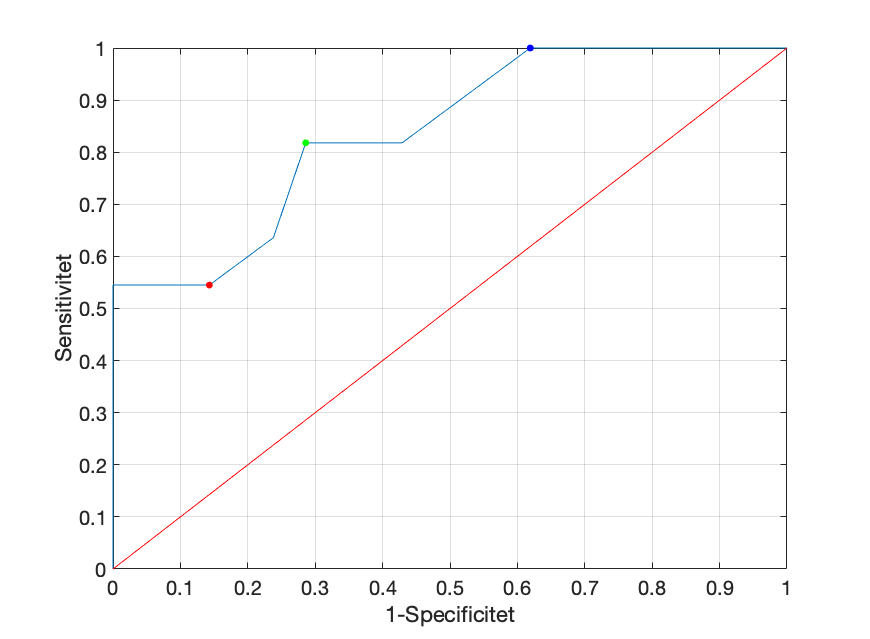
\includegraphics[width=1\textwidth]{billeder/ROC11.png} 
	\caption{ROC-kurve for sammenhængen mellem systemets sensitivitet og specificitet. På x-aksen er 1-specificitet angivet og på y-aksen sensitivitet. Den røde linje indikerer identitetslinjen og den blå linje ROC-kurven. Diskriminationsgrænser, er indikeret med en rød, grøn og blå prik.}
	\label{fig:ROC}  
\end{figure}

På Figur \ref{fig:ROC} fremgår det, at ROC-kurven, som er illustreret af den blå linje, er over identitetslinjen, som er illustreret af den røde linje, hvilket indikerer at systemet er god til at forudsige, hvornår lægemiddelskift kræver uddybende information. Derudover er dikriminationsgrænserne indikeret med en rød, grøn eller blå prik. For at understøtte systemets anvendelighed opsummeres nøjagtigheden af systemet ved at udregne arealet under kurven, hvilket fremgår af Tabel \ref{table:AUC}.

\begin{table}[H]
\caption{Arealet under kurven.}
\label{table:AUC}
\centering
\begin{tabular}{|l|l|l|l|l|} \hline
 \rowcolor[HTML]{C0C0C0} \textbf{Areal}  &  \textbf{Standard}                       & \textbf{Signifikant} &
 \multicolumn{2}{|c|}{\textbf{95 \% Konfidensinterval}}  \\ 
  \rowcolor[HTML]{C0C0C0}                                                          & \textbf{error} &  & Nedre grænse      & Øvre grænse    \\ \hline
0,840 & 0,074 & 0,002 & 0,696 & 0,984 \\ \hline
\end{tabular}
\end{table}
\vspace{0.1cm}

Af Tabel \ref{table:AUC} fremgår det, at arealet under kurven er 0,840 $\pm$ 0,074. Når en værdi på 1 antages at være en perfekt test~\citep{Greiner2000}, vurderes risikovurderingen til at være en god test til forudsigelse af, hvornår et lægemiddelskift kræver uddybende information, hvilket er statistisk signifikant (p=0,002). Derudover er 95~\% konfidensinterval for arealet under kurven for den nedre grænse på 0,696 og øvre grænse på 0,984. Dette indikerer, at ved en vurdering af 100 lægemiddelskift vil 95~\% af disse være inden for et interval på 0,696 og 0,984.

\section{Grænseværdier for risikovurdering}
Ud fra ROC-kurven på Figur \ref{fig:ROC}  er diskriminationsgrænser for risikoscoren undersøgt i forhold til at bestemme grænseværdier for, hvornår et lægemiddelskift kræver uddybende information. På Figur \ref{fig:ROC} er diskriminationsgrænsen for optimal balance mellem sensitiviteten og specificiteten, markeret med en grøn prik. Dette er opfyldt ved en sensitivitet på 0,818 og en 1-specificitet på 0,286, svarende til en specificitet på 0,714. Den røde prik indikerer en diskrimintationsgrænse med en sensitivitet på 0,545 og en 1-specificitet på 0,143, svarende til en specificitet på 0,455, hvor den blå prik indikerer en sensitivitet på 1,000 og en 1-specificitet på 0,619, svarende til en specificitet på 0,381. For diskriminationsgrænserne, svarende til den røde og grønne prik på Figur \ref{fig:ROC}, betyder dette, at der tillades en lavere sensitivitet og specificitet end for diskriminationgrænsen ved optimal balance. Dette betyder, at færre lægemiddelskift bliver identificeret korrekt i forhold til at kræve og ikke kræve uddybende information.


Ud fra diskriminationsgrænserne kan grænseværdier for risikoscoren bestemmes. Ud fra Tabel \ref{table:app_ROC} i Appendiks \ref{App:ROC} er diskriminationsgrænserne identificeret ved en risikoscore på  henholdsvis 7,5, 22,5 og 32,5~\%. Da grænseværdierne er angivet som gennemsnittet af to sammenhængende observerede værdier, defineres dette som den største værdi af de to observerede værdier. Dette gøres på baggrund af, at medarbejderne var enige i, at alle lægemiddelskift under en risikoscore på 10~\% ikke krævede uddybende information, jævnfør Tabel \ref{table:resultat} i Appendiks \ref{App:Resultat}. Derudover blev
lægemiddelskift med en risikoscore på 40~\% eller derover i gennemsnit vurderet af medarbejderne til at kræve uddybende information, hvilket fremgår af Tabel \ref{table:test2}. Dette vil sige, at grænseværdierne for risikoscoren er henholdsvis 10, 25 og 35~\%. Disse grænseværdier kan anvendes til at inddele lægemiddelskift ud fra risikoscoren i forhold til, hvor meget opmærksomhed lægemiddelskiftet kræver, hvilket er illustreret af Tabel~\ref{table:cutoff}.

\begin{table}[H]
\caption{Inddeling af lægemiddelskift ud fra risikoscore i forhold til, hvor meget opmærksomhed lægemiddelskiftet kræver.}
\vspace{2mm}
\label{table:cutoff} 
\centering
\begin{tabular}{|l|l|} \hline
\rowcolor[HTML]{C0C0C0}\textbf{Risikoscore} & \textbf{ Opmærksomhed} \\ \hline
\cellcolor[HTML]{C0C0C0} \textbf{<10~\%} & Ingen opmærksomhed \\ \hline
\cellcolor[HTML]{C0C0C0}\textbf{10-20~\%} & Begrænset opmærksomhed \\ \hline
\cellcolor[HTML]{C0C0C0}\textbf{25-35~\% }& Moderat opmærksomhed  \\ \hline
\cellcolor[HTML]{C0C0C0}\textbf{>35~\%} & Særlig opmærksomhed \\ \hline
\end{tabular}
\end{table}

Opdelingen af lægemiddelskift ud fra risikoscoren, som fremgår af Tabel~\ref{table:cutoff}, kan anvendes til at identificere lægemiddelskift ud fra, hvor meget opmærksomhed det enkelte lægemiddelskift kræver for implementering i klinikken. For lægemiddelskift under 10~\% kan disse sorteres fra i forhold til skiftelisterne, og de resterende lægemiddelskift kan markeres med en farveskala alt efter, hvor meget opmærksomhed de kræver. Dette kan f.eks. indikeres med grønt for begrænset opmærksomhed, gult for opmærksomhed og rødt for særlig opmærksomhed. På denne måde  kan farveindikationen anvendes som beslutningsstøtte for medarbejderne i forhold til at prioritere de enkelte lægemiddelskift og derved bruge mindre tid på lægemidelskift, som ikke kræver meget opmærksomhed og i stedet bruge tid på lægemiddelskift, hvor der kræves særlig opmærksomhed.

%\begin{figure} [H]
%	\centering
%	\begin{subfigure}{0.49\textwidth} % width of left subfigure
%		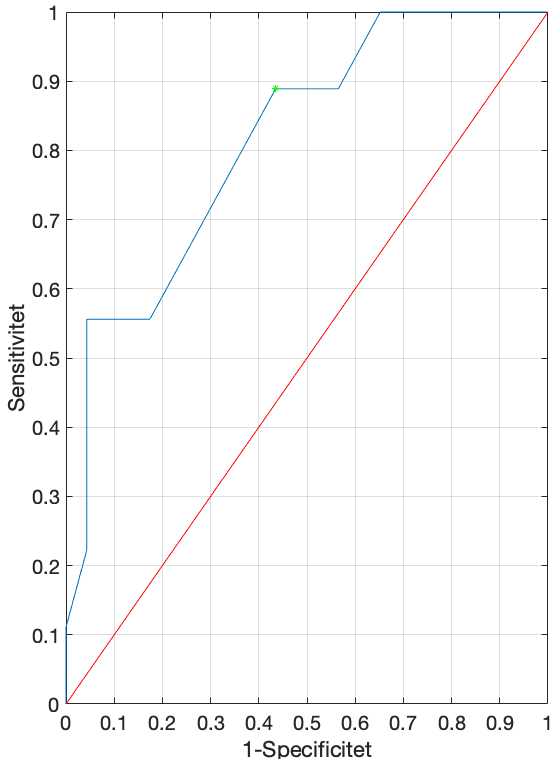
\includegraphics[width=\textwidth]{billeder/ROC.png}
%\subcaption{Lægemiddel Nyt. \label{fig:ROC1}}
%	\end{subfigure}
%	\vspace{1em}
%	\begin{subfigure}{0.49\textwidth} 
%		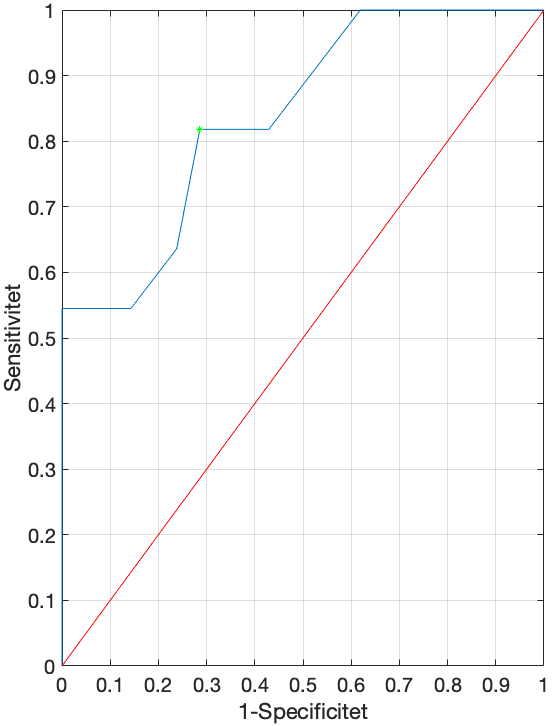
\includegraphics[width=\textwidth]{billeder/ROC1.png}
%\subcaption{Golden Standard. \label{fig:ROC2}}
%	\end{subfigure}
%	\vspace{-0.5cm}
%\caption{ROC-kurve for Lægemiddel Nyt på Figur \ref{fig:ROC1} og medarbejderne, angivet som Golden Standard, på Figur \ref{fig:ROC2}. På y-aksen er sensitivitet angivet og x-aksen 1-specificitet. Den røde linje indikerer identitetslinjen og den blå linje ROC-kurven. Diskriminationsgrænserne er indikeret med en grøn prik.}
%\label{fig:ROC}
%\end{figure} 
%
%På Figur \ref{fig:ROC} fremgår det, at ROC-kurven for Lægemiddel Nyt og medarbejderne, som er illustreret af den blå linje, er over identitetslinjen, som er illustreret af den røde. Derudover er diskriminationsgrænsen markeret med grøn, der hvor sensitiviteten og specificiteten er ligeværdige. For Lægemiddel Nyt er denne indikeret men en sensitivitet på 0,889 og 1-specificitet på 0,435, svarende til en specificitet på 0,565. For medarbejderne er diskriminationsgrænse indikeret ved en sensitivitet på 0,818 og en 1-specificitet på 0,286, svarende til en specificitet på 0,714. 
%
%Ved at sammenligne værdierne for sensitivitet og 1-specificitet med Tabel \ref{table:app_ROC} i Appendiks \ref{App:ROC} vil der ved en optimal balance mellem sensitivitet og specificitet ved en risikoscore på henholdsvis 17,5 for Lægemiddel Nyt og 22,5 for medarbejderne. 
%
%Ud fra diskriminationsgrænsen kan lægemiddelskiftene på baggrund af risikoscoren opdeles i forhold til lægemiddelskift, som kræver særlig opmærksomhed. Lægemiddelskift med en risikoscore på over 22,5, hvilket vil sige 30~\% og derover, kan markeres med rød farve i skiftelisterne, hvormed medarbejderne informeres om, at disse lægemiddelskift kræver særlig opmærksomhed. Ligeledes kan lægemiddelskift med en risikoscore på 15-20~\% markeres med gul farve i skiftelisterne, hvormed dette indikere at lægemiddelskiftet er kræver mindre opmærksomhed. Dernæst kan lægemiddelskift med en risikoscore på 0 til 10~\% indikeres med grøn i forhold til at disse kræver begrænset opmærksomhed ved implementering i klinikken.
%
%For at kunne vurdere nøjagtigheden af risikoscoren for både Lægemiddel Nyt og medarbejderne beregnes arealet under kurven, hvilket fremgår af Tabel \ref{table:AUC}.
%
%\begin{table}[H]
%\caption{Arealet under kurven for Lægemiddel Nyt og medarbejderne, angivet som Golden Standard.}
%\label{table:AUC}
%\centering
%\begin{tabular}{l|l|p{1.8cm}|l|l|l}
% \rowcolor[HTML]{C0C0C0}  &  &                         & \textbf{Signifikant} &
% \multicolumn{2}{c}{\textbf{95 \% Konfidensinterval}}  \\ 
%  \rowcolor[HTML]{C0C0C0}                                                         & \textbf{Areal} &  \textbf{Standard error}                       &  & Nedre grænse      & Øvre grænse    \\ \hline
%% \cellcolor[HTML]{C0C0C0}\textbf{ Lægemiddel Nyt }& 0,766 & 0,090 & 0,017 & 0,589 & 0,942  \\ \hline
% \cellcolor[HTML]{C0C0C0}\textbf{ Lægemiddel Nyt }& 0,841 & 0,082 & 0,006 & 0,653 & 0,975  \\ \hline
%\cellcolor[HTML]{C0C0C0} \textbf{Golden Standard} & 0,840 & 0,074 & 0,002 & 0,696 & 0,984 \\
%\end{tabular}
%\end{table}
%
%Af Tabel \ref{table:AUC} fremgår det at arealet under kurven er 0,841 for Lægemiddel Nyt og 0,840 for medarbejderne. I forhold til at antage at 1 er en perfekt test, vurderes risikoscoren for begge til at være god. Derudover er ROC-kurven statistisk signifikant for Lægemiddel Nyt (p=0,006) og Golden Standard (p=0,002). Lægemiddel Nyt har en nedre grænse på 0,653 og en øvre grænse på 0,975 af arealet under kurven, mens medarbejderne nedre grænse er på 0,696 og den øvre grænse er på 0,984. Dette vil sige, at ved en vurdering af 100 lægemiddelskiftet vil 95~\% af disse være mellem 0,589 og 0,942 for Lægemiddel Nyt og 0,696 og 0,984 for medarbejderne, hvilket vil sige, at lægemiddelskiftene vil befinde sig mellem en risikoscore på 12,5~\% og 27,5~\%.





%\section{Risikovurdering}
%Ud fra vurderingerne foretaget af 11 medarbejdere fra SRN er der defineret en Golden Standard. Denne er bestemt ud fra, at over 60~\% af medarbejderne var enige i at lægemiddelskiftet krævede uddybende information. Medarbejdernes vurdering sammenlignes med Lægemiddel Nyt i forhold til teste systemets sensitivitet og specificitet. Vurderingerne af, hvorvidt lægemiddelskift krævede uddybende information via Lægemiddel Nyt, ved sammenligning af Lægemiddel Nyt med Golden Standard for medarbejdernes vurdering fremgår af Tabel \ref{table:test1}, hvor de individuelle vurderinger af medarbejderne fremgår af Tabel \ref{table:resultat} i Appendiks \ref{App:Resultat}.
%
%\begin{table}[H]
%\caption{Vurderinger fra Lægemiddel Nyt og Golden Standard for medarbejderne i forhold til lægemiddelskift, som kræver uddybende information. Uenighed er markeret med gult og en vurdering under 60~\% enighed mellem medarbejderne er markeret med rødt.}
%\label{table:test1}
%\centering
%\begin{tabular}{l|c|c|c|c|c|c|c|c|c|c|c|c|c|c|c|c|c}
%\rowcolor[HTML]{C0C0C0} \textbf{} & \multicolumn{11}{|c|}{\textbf{Lægemiddelskift nummer}} \\
%\rowcolor[HTML]{C0C0C0} & \textbf{1} & \textbf{2} & \textbf{3} & \textbf{4} & \textbf{5} & \textbf{6} & \textbf{7} &  \textbf{8} & \textbf{9} & \textbf{10} & \textbf{11}   \\ \hline
%%\textbf{Risikoscore} & 0 & 0 & 5 & 5 & 5 & 5 & 5 & 5 & 10 & 10 & 10  \\ \hline
%\textbf{Lægemiddel Nyt} & nej & nej & nej & nej & nej & nej & nej & nej & ja &\cellcolor[HTML]{F6F6C3} ja & nej \\ \hline
%\textbf{Golden Standard} & nej & nej & nej& nej & nej &nej & nej & nej& ja & \cellcolor[HTML]{F6F6C3}nej & nej \\ \hline
%\rowcolor[HTML]{C0C0C0} & \multicolumn{11}{|c|}{\textbf{Lægemiddelskift nummer}} \\
%\rowcolor[HTML]{C0C0C0} & \textbf{12} & \textbf{13} & \textbf{14} &  \textbf{15} & \textbf{16} & \textbf{17} & \textbf{18} & \textbf{19} & \textbf{20} & \textbf{21} & \textbf{22}  \\ \hline
%%\textbf{Risikoscore} & 15 & 15 & 15 & 15 & 20 & 20 & 20 & 25 & 25 & 25 & 30 \\ \hline
%\textbf{Lægemiddel Nyt} & nej & nej & \cellcolor[HTML]{F6F6C3}nej & nej & nej & nej & \cellcolor[HTML]{F6F6C3}ja & \cellcolor[HTML]{F6F6C3}nej & \cellcolor[HTML]{F6F6C3}ja & \cellcolor[HTML]{F6F6C3}nej & \cellcolor[HTML]{F6F6C3}nej\\ \hline
%\textbf{Golden Standard} & \cellcolor[HTML]{F6E6E5} - & nej & \cellcolor[HTML]{F6F6C3}ja & nej & nej & nej & \cellcolor[HTML]{F6F6C3}nej & \cellcolor[HTML]{F6F6C3}ja & \cellcolor[HTML]{F6F6C3}nej & \cellcolor[HTML]{F6F6C3}ja & \cellcolor[HTML]{F6F6C3}ja \\ \hline
%\rowcolor[HTML]{C0C0C0} & \multicolumn{11}{|c|}{\textbf{Lægemiddelskift nummer}} \\ 
%\rowcolor[HTML]{C0C0C0} & \textbf{23} & \textbf{24} & \textbf{25} & \textbf{26} & \textbf{27} & \textbf{28} &  \textbf{29} & \textbf{30} & \textbf{31} & \textbf{32} & \textbf{33}  \\ \cline{1-10}
%\textbf{Lægemiddel Nyt} & nej & \cellcolor[HTML]{F6F6C3}ja & nej & nej & nej & ja & ja & ja & ja & \cellcolor[HTML]{F6F6C3}nej & ja\\ \hline
%\textbf{Golden Standard} & nej & \cellcolor[HTML]{F6F6C3}nej & nej & nej & nej & ja & ja& ja & ja& \cellcolor[HTML]{F6F6C3}ja & ja \\\hline
%\end{tabular}
%\end{table}
%
%Det fremgår af Tabel \ref{table:test1}, at der ikke er en 60~\% enighed mellem medarbejderne i forhold til lægemiddelskift nummer 12, hvorfor dette lægemiddelskift undlades i den efterfølgende databehandling. En medarbejder kommenterede i forhold til dette lægemiddelskift, at begrundelsen for lægemiddelskiftet ikke var dækkende, hvilket fremgår af Tabel \ref{table:resultat2} i Appendiks \ref{App:Resultat}. Af Tabel \ref{table:test1} fremgår det, at der er uenighed mellem Lægemiddel Nyt og medarbejdernes vurdering for 9 lægemiddelskift svarende til 27~\% og enighed for 23, svarende til 69,7~\%. 
%For at undersøge systemets nøjagtighed i forhold til Golden Standard beregnes sensitivitet og specificitet, hvilket fremgår af Tabel \ref{table:PositivNegativ}.
%
%\begin{table}[H]
%\caption{Krydstabel for Lægemiddel Nyt og Golden Standard for medarbejderne. Sensitiviteten er markeret med blåt og specificiteten er angivet med grønt.}
%\label{table:PositivNegativ}
%\centering
%\begin{tabular}{ll|l|l|l|l}
% \rowcolor[HTML]{C0C0C0}                          &                          &                            & \multicolumn{2}{c|}{\textbf{Golden Standard}} &        \\ 
%  \rowcolor[HTML]{C0C0C0}                                                         &                          &                            & Positiv       & Negativ          & Antal  \\ \hline
%\cellcolor[HTML]{C0C0C0} \textbf{Lægemiddel}                                                \hspace{-0.5cm} \multirow{4}{*}{} &  \cellcolor[HTML]{C0C0C0}                                                      Positiv \multirow{2}{*}{} & Antal & 6                & 4                & 10     \\ \cline{3-6} 
%\cellcolor[HTML]{C0C0C0}                                                                \textbf{Nyt} &   \cellcolor[HTML]{C0C0C0}                                               & \% indenfor Golden Standard & \cellcolor[HTML]{ECF4FF} 54,5 \%           & 19,0 \%           & 31,3 \% \\\cline{2-6}
%\cellcolor[HTML]{C0C0C0}                                                                                 & \cellcolor[HTML]{C0C0C0}                                                                               Negativ \multirow{2}{*}{} & Talte & 5                & 17               & 22     \\ \cline{3-6}
%          \cellcolor[HTML]{C0C0C0}                                                                             &                         \cellcolor[HTML]{C0C0C0}                                                        & \% indenfor Golden Standard & 45,5 \%           & \cellcolor[HTML]{D4EED3}81,0 \%            & 68,8 \% \\ \hline
% \cellcolor[HTML]{C0C0C0}                                                                            \textbf{Total}                         &                          \cellcolor[HTML]{C0C0C0}                                                                             & Antal                     & 11               & 21               & 32     \\ \cline{3-6}
%                          \cellcolor[HTML]{C0C0C0}                                                                                   &                           \cellcolor[HTML]{C0C0C0}                                                                            & \% indenfor Golden Standard & 100 \%            & 100\%            & 100 \% 
%\end{tabular}
%\end{table}
%
%Af Tabel \ref{table:PositivNegativ} fremgår det, at lægemiddelskiftet blev vurderet positiv, hvilket vil sige, at der var enighed mellem Lægemiddel Nyt og medarbejderne vurdering i 6 tilfælde. Ligeledes  blev lægemiddelskiftet i 21 tilfælde vurderet negativt af både Lægemiddel Nyt og medarbejderne, hvilket vil sige at der var enighed om at lægemiddelskiftet ikke krævede uddybende informationer. Lægemiddelskiftet blev i 5 tilfælde vurderet negativt af Lægemiddel Nyt og positivt af medarbejderne, mens det i 4 tilfælde blev vurderet positivt af Lægemiddel Nyt, men negativt af medarbejderne. 
%
%Ud fra Tabel \ref{table:PositivNegativ} fremgår det ligeledes at systemets sensitivitet er 54,5~\% og sensitivitet er 81~\%.  Dette vil sige, at systemet i 54,5~\% af tilfældene vil foretage en korrekt vurdering af at et lægemiddelskift kræver uddybende information, og i 81~\% af tilfældene vil foretage en korrekt vurdering af at et lægemiddelskift ikke kræver uddybende information. Derudover vil systemt i 45,5~\% af tilfældene give anledning til type 2 fejl, hvilket vil sige, at systemet vil vurdere at et lægemiddelskift ikke kræver uddybende information, hvor dette var tilfældet. Yderligere vil systemet i 19~\% af tilfældene give anledning til type 1 fejl, hvor systemet vil vurdere at et lægemiddelskift som ikke kræver uddybende information vil blive vurderet til at kræve dette.
%
%For at undersøge overensstemmelsen mellem Lægemiddel Nyt og Golden Standard bestemmes Cohen's kappa-koefficienten, hvilket fremgår af Tabel \ref{table:Kappa}.
%
%\begin{table}[H]
%\caption{Cohen's kappa analyse}
%\label{table:Kappa}
%\centering
%\begin{tabular}{l|l|l|l}
% \rowcolor[HTML]{C0C0C0}  &  \textbf{Værdi} &   \textbf{Standard Error} & \textbf{Signifikant} \\ 
%  \cellcolor[HTML]{C0C0C0}                                                       \textbf{Kappa} & 0,363 & 0,174 & 0,040 \\
%\end{tabular}
%\end{table}
%
%Af Tabel \ref{table:Kappa} fremgår det at kappa-koefficienten er 0,363, hvilket vil sige at overensstemmelsen mellem Lægemiddel Nyt og Golden Standard er begrænset, hvis det antages at en perfekt overensstemmelse er svarende til 1. Derudover fremgår det at resultatet er signifikant (p=0,040).

%\section{Risikoscore}
%Ud af 33 lægemidler blev 19 lægemiddelskift  vurderet til at skulle have enten lavere eller højere risikoscore end systemet havde udregnet af én eller flere medarbejdere, hvilket fremgår af Tabel \ref{table:resultat3} i Appendiks \ref{App:Rang}. Ud af vurderinger fra 6 medarbejdere var der enighed mellem 4 i forhold til  at 2 ud af 33 lægemiddelskift krævede lavere risikoscore. For at evaluere risikoscoren sammenlignes vurderingerne af Lægemiddel Nyt og medarbejderne angivet som Golden Standard med den beregnede risikoscore for lægemiddelskiftene, hvilket fremgår af Tabel \ref{table:test2}.
%
%\begin{table}[H]
%\caption{Risikoscore og vurdering af lægemiddelskift for Lægemiddel Nyt og medarbejderne fra SRN, angivet som Golden Standard. Vurdering under 60~\% enighed mellem medarbejderne er markeret med rødt.}
%\label{table:test2}
%\centering
%\begin{tabular}{l|c|c|c|c|c|c|c|c|c|c|c|c|c|c|c|c|c}
%\rowcolor[HTML]{C0C0C0} \textbf{} & \multicolumn{11}{|c}{\textbf{Lægemiddelskift nummer}} \\
%\rowcolor[HTML]{C0C0C0} & \textbf{1} & \textbf{2} & \textbf{3} & \textbf{4} & \textbf{5} & \textbf{6} & \textbf{7} &  \textbf{8} & \textbf{9} & \textbf{10} & \textbf{11}   \\ \hline
%\textbf{Risikoscore [\%]} & 0  & 0 & 5 & 5 & 5 & 5 & 5 & 5 & 10 & 10 & 10  \\ \hline
%\textbf{Lægemiddel Nyt} & nej & nej & nej & nej & nej & nej & nej & nej & ja & ja & nej \\ \hline
%\textbf{Golden Standard} & nej & nej & nej& nej & nej &nej & nej & nej& ja & nej & nej \\ \hline
%\rowcolor[HTML]{C0C0C0} & \multicolumn{11}{|c}{\textbf{Lægemiddelskift nummer}} \\
%\rowcolor[HTML]{C0C0C0} & \textbf{12} & \textbf{13} & \textbf{14} &  \textbf{15} & \textbf{16} & \textbf{17} & \textbf{18} & \textbf{19} & \textbf{20} & \textbf{21} & \textbf{22}  \\ \hline
%\textbf{Risikoscore [\%]} & \cellcolor[HTML]{F6E6E5} 15 & 15 & 15 & 15 & 20 & 20 & 20 & 25 & 25 & 25 & 30 \\ \hline
%\textbf{Lægemiddel Nyt} & \cellcolor[HTML]{F6E6E5}nej & nej & nej & nej & nej & nej & ja & nej & ja & nej & nej\\ \hline
%\textbf{Golden Standard} & \cellcolor[HTML]{F6E6E5} - & nej & ja & nej & nej & nej & nej & ja & nej & ja & ja \\ \hline
%\rowcolor[HTML]{C0C0C0} & \multicolumn{11}{|c}{\textbf{Lægemiddelskift nummer}} \\ 
%\rowcolor[HTML]{C0C0C0} & \textbf{23} & \textbf{24} & \textbf{25} & \textbf{26} & \textbf{27} & \textbf{28} &  \textbf{29} & \textbf{30} & \textbf{31} & \textbf{32} & \textbf{33}  \\ \cline{1-10}
%\textbf{Risikoscore [\%]} & 30 & 30 & 35 & 35 & 35 & 40 & 40 & 45 & 50 & 50 & 55 \\ \hline 
%\textbf{Lægemiddel Nyt} & nej & ja & nej & nej & nej & ja & ja & ja & ja & nej & ja\\ \hline
%\textbf{Golden Standard} & nej & nej & nej & nej & nej & ja & ja& ja & ja&ja & ja \\\hline
%\end{tabular}
%\end{table}
%
%Ud fra Tabel \ref{table:test2} fremgår det, at der ved lægemiddelskift nummer 12 var under 60~\% enighed mellem medarbejderne, hvormed dette skift ikke tages med i den videre databehandling.  
%Derudover fremgår det, at lægemiddelskift med en risikoscore på 10, 20, 25, 30 og 50 \% er vurderet forskelligt af Lægemiddel Nyt i forhold til uddybende information, hvor en risikoscore på 10, 15, 25 og 30 \% er vurderet forskelligt af medarbejderne fra SRN. For lægemiddelskift med en risikoscore mellem 0 og 5~\% er der enighed mellem medarbejderne, hvilket fremgår af Tabel \ref{table:resultat}. Denne enighed gør sig også gældende mellem Lægemiddel Nyt og medarbejderne. 
%
%Lægemiddelskift nummer 9 og 14, med en risikoscore på henholdsvis 10 og 15 \%, er vurderet anderledes end de resterende med samme risikoscore. For disse lægemiddelskift var der angivet kommentarer i forhold til uenighed om, hvorvidt styrken eller styrkeangivelsen var ændret, hvilket fremgår af Tabel \ref{table:resultat2} i Appendiks \ref{App:Resultat}. Ligeledes blev lægemiddelskift nummer 22, med en risikoscore på 30~\%, vurderet anderledes end de andre med samme risikoscore. En medarbejder kommenterede i forhold til dette, at ATC-koden i dette tilfælde vil være mindre kritisk sammenlignet med andre.
%
%For at undersøge systemets diskriminationsgrænse i forhold til at definere den bedste grænse for, hvornår et lægemiddelskift kræver uddybende information ud fra risikoscoren er sensitiviteten som funktion af 1-specificiteten for hver risikoscore udregnet, hvilket fremgår af Tabel \ref{table:app_ROC} i Appendiks \ref{App:ROC}, og visualiseret via ROC-kurven, som fremgår af Figur \ref{fig:ROC}. 
%
%\begin{figure} [H]
%	\centering
%	\begin{subfigure}{0.49\textwidth} % width of left subfigure
%		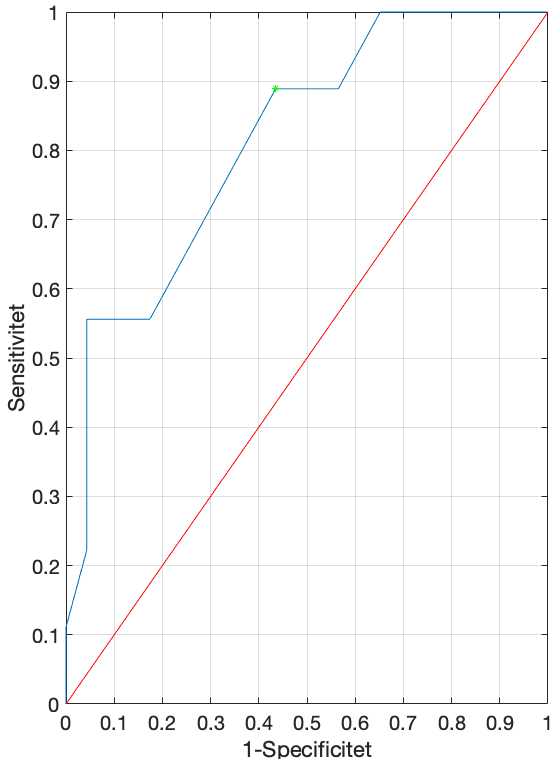
\includegraphics[width=\textwidth]{billeder/ROC.png}
%\subcaption{Lægemiddel Nyt. \label{fig:ROC1}}
%	\end{subfigure}
%	\vspace{1em}
%	\begin{subfigure}{0.49\textwidth} 
%		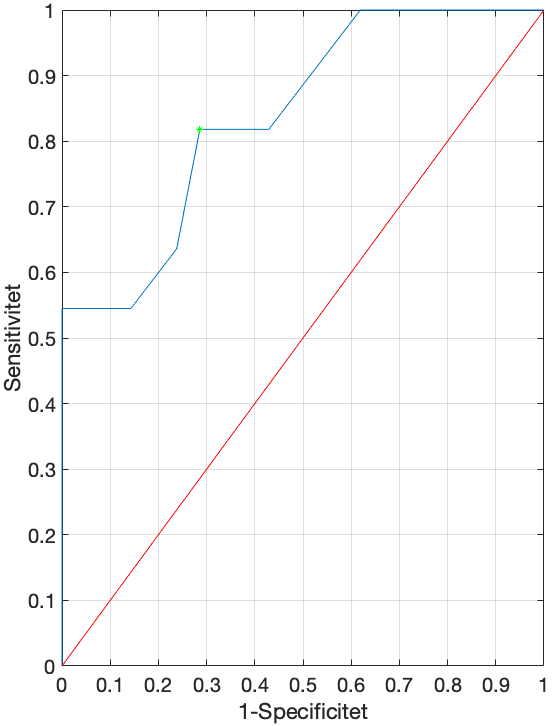
\includegraphics[width=\textwidth]{billeder/ROC1.png}
%\subcaption{Golden Standard. \label{fig:ROC2}}
%	\end{subfigure}
%	\vspace{-0.5cm}
%\caption{ROC-kurve for Lægemiddel Nyt på Figur \ref{fig:ROC1} og medarbejderne, angivet som Golden Standard, på Figur \ref{fig:ROC2}. På y-aksen er sensitivitet angivet og x-aksen 1-specificitet. Den røde linje indikerer identitetslinjen og den blå linje ROC-kurven. Diskriminationsgrænserne er indikeret med en grøn prik.}
%\label{fig:ROC}
%\end{figure} 
%
%På Figur \ref{fig:ROC} fremgår det, at ROC-kurven for Lægemiddel Nyt og medarbejderne, som er illustreret af den blå linje, er over identitetslinjen, som er illustreret af den røde. Derudover er diskriminationsgrænsen markeret med grøn, der hvor sensitiviteten og specificiteten er ligeværdige. For Lægemiddel Nyt er denne indikeret men en sensitivitet på 0,8 og 1-specificitet på 0,455, svarende til en specificitet på 0,545. Medarbejdernes diskriminationsgrænse er indikeret ved en sensitivitet på 0,818 og en 1-specificitet på 0,286, svarende til en specificitet på 0,714. Ved at sammenligne disse værdier med Tabel \ref{table:app_ROC} i Appendiks \ref{App:ROC} indikerer dette et cut-off på henholdsvis 17,5 for Lægemiddel Nyt og 22,5 for medarbejderne. Dette vil sige, at i tilfælde af, at scoren er under denne cut-off vil dette betyde, at der ikke skal være uddybende information til klinikken, mens en cut-off over denne værdi vil betyde at lægemiddelskiftet kræver uddybende information til klinikken. \textcolor{red}{Er lidt i tvivl om, hvordan jeg skal definere balancen mellem sensitivitet og specificitet. Synes det er vigtigt at alle lægemidler som kræver uddybende information bliver uddybet, så en høj sensitivitet, men at lægemidler som ikke kræver uddybende information bliver uddybet har ikke så stor betydning, så lav specificitet.}
%
%For at kunne vurdere nøjagtigheden af risikoscoren for både Lægemiddel Nyt og medarbejderne beregnes arealet under kurven, hvilket fremgår af Tabel \ref{table:AUC}.
%
%\begin{table}[H]
%\caption{Arealet under kurven for Lægemiddel Nyt og medarbejderne, angivet som Golden Standard.}
%\label{table:AUC}
%\centering
%\begin{tabular}{l|l|p{1.8cm}|l|l|l}
% \rowcolor[HTML]{C0C0C0}  &  &                         & \textbf{Signifikant} &
% \multicolumn{2}{c}{\textbf{95 \% Konfidensinterval}}  \\ 
%  \rowcolor[HTML]{C0C0C0}                                                         & \textbf{Areal} &  \textbf{Standard error}                       &  & Nedre grænse      & Øvre grænse    \\ \hline
% \cellcolor[HTML]{C0C0C0}\textbf{ Lægemiddel Nyt }& 0,766 & 0,090 & 0,017 & 0,589 & 0,942  \\ \hline
% \cellcolor[HTML]{C0C0C0} \textbf{Golden Standard} & 0,840 & 0,074 & 0,002 & 0,696 & 0,984 \\
%\end{tabular}
%\end{table}
%
%Af Tabel \ref{table:AUC} fremgår det at arealet under kurven er 0,766 for Lægemiddel Nyt og 0,840 for medarbejderne. I forhold til at antage at 1 er en perfekt test, vurderes risikoscoren for Lægemiddel Nyt til at være rimelig og medarbejderne til at være god. Derudover er ROC-kurven statistisk signifikant for Lægemiddel Nyt (p=0,017) og Golden Standard (p=0,002). Lægemiddel Nyt har en nedre grænse på 0,589 og en øvre grænse på 0,942 af arealet under kurven, hvilket vil sige, at ved en vurdering af 100 lægemiddelskiftet vil 95~\% af disse være mellem 0,589 og 0,942. For medarbejderne er denne nedre grænse på 0,696 og den øvre grænse på 0,984 af arealet under kurven, dette vil sige, at 95~\% af konfidensintervallet ligger mellem 0,696 og 0,984.


%\section{Systemets performance}
%Ud af lægemiddelskiftene var der for 13 lægemidler enighed mellem medarbejderne fra SRN. Ud af 33 blev 11 lægemidler vurderet til ikke at krævede uddybende samt at 2 lægemidler krævede uddybende information ved implementering af disse i klinikken. Størstedelen af lægemiddelskift blev vurderet af 9 ud af 11 til ikke at kræve uddybende information, mens 2 medarbejdere vurderede at størstedelen af lægemidlerne krævede uddybende information, hvilket er markeret med blåt i Tabel \ref{table:test1}. Gennemsnittet blev vurderet til at 12,27 lægemidler, svarende til 37,19~\%, krævede uddybende information, mens 20,63 lægemidler, svarende til 62,5~\%, ikke krævede uddybende information, hvilket ligeledes fremgår af Tabel \ref{table:test1}. 

%\begin{table}[H]
%\caption{Krydstabel for vurderingen ja eller nej i forhold til uddybende information om lægemiddelskiftet og testpersoner samt lægemiddel Nyt, som er indikeret som nummer 12. \textcolor{red}{Er i tvivl, hvorvidt det giver mening at have lægemiddel Nyt med i denne test}}
%\vspace{2mm}
%\label{table:test1}
%\centering
%\begin{tabular}{l|c|c|c|c|c|c|c|c|c|c|c|c|c}
%\rowcolor[HTML]{C0C0C0}
% & \multicolumn{11}{|c|}{\textbf{Testperson}} & \textbf{} & \textbf{Total}    \\
%\rowcolor[HTML]{C0C0C0}  & \textbf{1}  & \textbf{2}  & \textbf{3} & \textbf{4} & \textbf{5} & \textbf{6} & \textbf{7} & \textbf{8} & \textbf{9} & \textbf{10} & \textbf{11} & \textbf{12}  & \\ 
%\cellcolor[HTML]{C0C0C0}{Antal af Nej}            & 24 & 20 & 21  &  28 &  15 &  21 & 17   &  12  & 21  & 26   &  22  & 29 & 256      \\ \cline{2-13}
%\cellcolor[HTML]{C0C0C0}{\% af Nej }  & 9,4 & 7,8  & 8,2 & 10,9  & 5,9  &  8,2 & 6,6  & 4,7  & 8,2 & 10,2  &  8,6 & 11,3 &  100    \\ \cline{2-13}
%\cellcolor[HTML]{C0C0C0}{\% af Gruppe} & 72,7 &  60,6  & 63,6 & 84,8   & 45,5   & 63,6  & 51,5  & 36,4 & 63,6 & 78,8 & 66,7  & 87,9 & 64,6 \\ \cline{2-13}
%\cellcolor[HTML]{C0C0C0}{\% af Total}  & 6,1 & 5,1 & 5,3  & 7,1 & 3,8 & 5,3  & 4,3 & 3,0  & 5,3 & 6,6  & 5,6  & 7,3 &  64,6 \\ \hline
%\cellcolor[HTML]{C0C0C0}{Antal af Ja} & 9 & 13 & 12 & 5  &  \cellcolor{blue}{18} & 12  & 16  &  \cellcolor{blue}{21}  & 12 & 7  & 11 & 4 & 140    \\ \cline{2-13} \cellcolor[HTML]{C0C0C0}{\% af Ja}  & 6,4 & 9,3  & 8,6 & 3,6 & 12,9  & 8,6  & 11,4 & 15  & 8,6  & 5,0 & 7,9  & 2,9 & 100   \\ \cline{2-13}
% \cellcolor[HTML]{C0C0C0}{\% af Gruppe} & 27,3 & 39,4 & 36,4 & 15,2   & 54,5  & 36,4 & 48,5 & 63,6  & 36,4 & 21,2 & 33,3  & 12,1 & 35,4      \\ \cline{2-13}
%\cellcolor[HTML]{C0C0C0}{\% af Total}  & 2,3   & 3,3 & 3,0 & 1,3 & 4,5 & 3,0 & 4,0 & 5,3 & 3,0 & 1,8 &  2,8  & 1,0 &  35,4     \\ \hline  \cellcolor[HTML]{C0C0C0}{Total}  & 33 & 33 & 33  & 33  & 33  & 33  & 33  &  33 &  33 &   33 &  33  &  33 &  396     \\ \cline{2-13}
% \cellcolor[HTML]{C0C0C0}{\% af Nej og Ja}  & 8,3    & 8,3    &  8,3  & 8,3   &  8,3  &  8,3  &  8,3  &  8,3  & 8,3   & 8,3    & 8,3    &  8,3 &  100    \\ \cline{2-13}
% \cellcolor[HTML]{C0C0C0}{\% af Gruppe} & 100   & 100   &  100 &  100 &  100 &  100 &  100 & 100  & 100  & 100   &  100  & 100 &      100 \\ \cline{2-13}
%\cellcolor[HTML]{C0C0C0}{\% af Total} & 8,3    & 8,3    &  8,3  & 8,3   &  8,3  &  8,3  &  8,3  &  8,3  & 8,3   & 8,3    & 8,3    &  8,3 &  100   \\
%\end{tabular}
%\end{table}

%For alle lægemiddelskift med en risikoscore på enten 0 eller 5~\% blev det vurderet at uddybende information var unødvendigt, hvilket vil sige at ændring i navn alene kræver mindre opmærksomhed, hvilket er illustreret af Tabel \ref{table:risikofaktorer}. Derudover var 10 ud af 11 medarbejdere enige i at lægemidler, hvor styrken alene eller i kombination med ændring i navn krævede uddybende information til klinikken. De medarbejdere som var uenige kommenterede at styrkeangivelsen var ændret, men at selve styrken ikke var ændret. Derimod blev ændring i dispenseringsform alene ikke vurderet lige så nødvendig at give uddybende information som ved styrke. Vurderingen i forhold til hvorvidt der kræves uddybende information ved ændringer i navn, styrke og dispenseringsform eller en kombination af disse fremgår af Tabel \ref{table:risikofaktorer}.

%\begin{table}[H]
%\caption{Oversigt over risikofaktorer og kombination mellem disse i forhold til uddybende information omkring lægemiddelskift (Ja = uddybende information, nej = ikke uddybende information).}
%\vspace{2mm}
%\label{table:risikofaktorer}
%\centering
%\begin{tabular}{l c|c|c|c}
%\rowcolor[HTML]{C0C0C0} & & \multicolumn{3}{c}{\textbf{I kombination med}} \\
%\rowcolor[HTML]{C0C0C0} & & \textbf{Navn}& \textbf{Styrke} & \textbf{Dispenseringsform} \\
%\cellcolor[HTML]{C0C0C0} & \cellcolor[HTML]{C0C0C0}Ja & 0 & 9.5 & 7 \\ \cline{2-5}	   
%\multirow{-2}{*}{\cellcolor[HTML]{C0C0C0}\textbf{Navn}} & \cellcolor[HTML]{C0C0C0}Nej & 11 & 1.5 & 4\\ \hline 
%\cellcolor[HTML]{C0C0C0} &  \cellcolor[HTML]{C0C0C0}Ja & 9.5 & 10 & 9.5 \\ \cline{2-5}	   
%\multirow{-2}{*}{\cellcolor[HTML]{C0C0C0}\textbf{Styrke}} & \cellcolor[HTML]{C0C0C0}Nej & 1.5 & 1 & 1.5\\ \hline 
%\cellcolor[HTML]{C0C0C0} & \cellcolor[HTML]{C0C0C0}Ja & 7 & 9.5 & 3.5 \\ \cline{2-5}	   
%\multirow{-2}{*}{\cellcolor[HTML]{C0C0C0}\textbf{Dispenseringsform}} & \cellcolor[HTML]{C0C0C0}Nej & 4 & 1.5 & 7.5 \\ \hline 
%\end{tabular}
%\end{table}

%Af Tabel \ref{table:risikofaktorer} fremgår det at, hvis styrken er ændret vil dette som udgangspunkt være den risikofaktorer, der oftest kræver uddybende information, både alene eller i kombination med enten navn eller dispenseringsform. Ændring i dispenseringsform blev i sjældnere tilfælde end styrke, vurderet til at kræve uddybende information og denne vurdering steg hvis ændring i dispenseringsform blev kombineret med navn eller styrke. Ændring i navn kræver kun uddybende information i kombination med styrke eller dispenseringsform. 

%Ud af 11 medarbejdere var 10 enige i at lægemiddelskift, hvor ATC-koden var angivet som kritisk eller at lægemidlet indgår i Medicinrådets behandlingsvejledning alene ikke krævede uddybende information til klinikken. Kommentarer fra de som var uenige med størstedelen var at et lægemiddelskift, som indgår i Medicinrådets behandlingsvejledning ikke nødvendigvis er kritisk, men at ændringer i behandlingsvejledning kan gøre lægemiddelskiftet kritisk. Derudover blev det vurderet at look-a-like alene og i kombination med navn ikke have indflydelse på om lægemiddelskiftet krævede uddybende information. I forhold til dette blev der kommenteret at look-a-like som udgangspunkt ikke er et problem, men kan opstå ved variationer af lægemidlets navn, hvor dette får betydning for ændringer ved dispenseringsformer.

%Rækkefølgen på lægemiddelskiftene som er vurderet på baggrund af risikoscoren blev vurderet af 6 ud af de 11 medarbejdere. Ud af 33 lægemiddelskift blev 18 lægemidler vurderet af én eller flere til at skulle rangeres lavere end systemet. Ud af de 6 medarbejdere var 4 eller 3 enige i at henholdsvis 2 eller 3 lægemidler skulle rangeres lavere end systemet.

%\section{Systemets brugbarhed}
%Systemet blev vurderet som et brugbart hjælpeværktøj i forhold til at oplysninger om lægemiddelskiftet kan genereres automatisk, hvormed der kan bruges mindre tid på helt simple skift. Dog skal systemet ikke overtage, da erfaringen inden for området stadig har stor betydning for risikovurderingen af lægemiddelskift. 

%Det blev vurderet at funktioner, såsom Look-a-like og Medicinrådet, ikke nødvendigvis skulle vægtes så højt, da det afhænger af den enkelte situation. Look-a-like vægtes generelt ikke særligt højt i den nuværende vurdering af lægemiddelskift varetaget af medarbejdere fra SRN, hvoraf antallet af egenskaber der skifter er mere afgørende for kompleksiteten såsom holdbarhed, emballage og konserveringsmidler. I forhold til Medicinrådet blev det vurderet at det ikke var vigtigt, hvorvidt lægemidlet indgik i Medicinrådets behandlingsvejledning, men hvorvidt der var foretaget ændringer i denne havde større betydning. 

%I forhold til videreudvikling blev det vurderet at systemet skal have flere problemstillinger som input, såsom pris i forhold til hvor meget det koster og hvor meget der forbruges samt hvor mange patienter og afdelinger som anvender lægemidlet. Derudover bør granuleringen af look-a-like, navneændring og dispenseringsform i forhold til vægtningen af risikoscoren overvejes. Nogle ændringer i navn og dispenseringsform vil kunne ligestilles og derfor ikke have betydning for klinikken, hvis der skiftes mellem disse. Der skal ligeledes skelnes mellem styrke og styrkeangivelse, da ændringerne ved styrkeangivelse ikke vil have en betydning, hvis pakningsstørrelsen ikke er ændret. Systemets anvendelighed blev derudover perspektiveret i forhold til at kunne anvendes til andre processer i forbindelse med lægemiddelskift såsom at anvende et lignende systemet ved udbud på lægemidler inden de endelige lægemiddelskift er vedtaget. 



